%---------- Inleiding ---------------------------------------------------------

\section{Introductie}%
\label{sec:introductie}
\section{Inleiding}

Dit onderzoek richt zich op het optimaliseren van het patchmanagement in groot- en middelgrote bedrijven die gebruikmaken van SAP ERP-systemen (Enterprise resource planning). ERP-software speelt een essentiële rol in bedrijfsomgevingen, geïllustreerd door het brede gebruik ervan, waarbij 62\% van de ondernemingen met minstens 10 werknemers in 2021 ERP-software implementeerde, volgens recente gegevens \autocite{Statistiek Vlaanderen}.

De doelgroep van dit onderzoek bestaat uit IT-professionals en organisaties die gebruikmaken van SAP ERP-systemen, met een focus op groot- en middelgrote bedrijven. In plaats van een algemene benadering, zullen we ons concentreren op een specifieke probleemsituatie binnen deze doelgroep. Het onderwerp wordt nauwkeurig afgebakend om vanuit een casus een concrete oplossing te bieden, in lijn met het toegepaste karakter van een bachelorproef.

De probleemstelling komt voort uit de uitdagingen waarmee organisaties worden geconfronteerd bij het effectief beheren van ERP-downtime en het toepassen van patches in SAP ERP-systemen. Trage updates, compatibiliteitsproblemen en mogelijke verstoring van bedrijfsactiviteiten zijn enkele van de veelvoorkomende obstakels in het patchmanagementproces. De noodzaak om patches tijdig toe te passen, met name voor het aanpakken van beveiligingskwetsbaarheden, wordt nog verder geaccentueerd door de alarmerende toename van ransomware-aanvallen, zoals blijkt uit het feit dat alleen al in 2021 623,3 miljoen van dergelijke aanvallen werden geregistreerd \autocite{Griffiths2022}.

De centrale onderzoeksvraag van dit onderzoek luidt: "Hoe kan het patchmanagement van ERP-systemen geoptimaliseerd worden in groot- en middelgrote bedrijven die gebruikmaken van SAP ERP?" Het doel van dit onderzoek is het ontwikkelen van een holistisch begrip van de bestaande patchmanagementpraktijken, de invloed van trends in SAP ERP, en de keuze tussen handmatig en automatisch patchen. 

De onderzoeksdoelstelling is het bieden van concrete inzichten die zullen resulteren in conclusies en aanbevelingen om het ERP- patchmanagement te optimaliseren. Het verwachte eindresultaat is niet alleen een uitgeschreven scriptie, maar ook een praktisch toepasbaar resultaat zoals een rapport met aanbevelingen voor het specifieke bedrijf dat als casus dient. Het succes van dit onderzoek wordt gemeten aan de hand van de effectiviteit van de voorgestelde optimalisatiemaatregelen en de implementeerbaarheid van de aanbevelingen in de bedrijfscontext.

\subsection{Deelvragen}
- Wat zijn de bestaande patchmanagementpraktijken in groot- en middelgrote bedrijven? \\
- Welke uitdagingen en succesfactoren worden geïdentificeerd in het huidige patchmanagementproces? \\
- Wat zijn de belangrijkste trends en ontwikkelingen in SAP ERP en patchmanagement? \\
- Hoe worden opkomende technologische trends zoals cloud computing en IoT verwacht invloed te hebben op patchmanagement? \\
- Hoe beïnvloeden menselijke, technologische en organisatorische factoren de efficiëntie van patchmanagement? \\
- Welke strategieën kunnen worden toegepast om de impact op de operationele continuïteit te minimaliseren? \\
- Welke communicatiestrategieën zijn essentieel voor het informeren van belanghebbenden over patchingactiviteiten? \\

\section{State-of-the-art}%
\label{sec:state-of-the-art}

\subsection{ERP Integratie}
Het domein van ERP-downtime en patchmanagement binnen SAP ERP-systemen is complex en dynamisch, met een voortdurende evolutie van technologieën en bedrijfsbehoeften. In een studie van \autocite{StatistiekVlaanderen2022} wordt de enorme integratie van ERP-software in bedrijfsomgevingen in België benadrukt, waaruit blijkt dat 62 \% van de ondernemingen met minstens 10 werknemers in 2021 ERP-software gebruikte. Deze statistiek geeft aan dat ERP-software, die zorgt voor een geautomatiseerde gegevensuitwisseling tussen verschillende afdelingen, een essentieel instrument is geworden voor het delen van informatie binnen bedrijven. Bovendien blijkt uit de gegevens dat grotere ondernemingen vaker gebruik maken van ERP-software, waarbij maar liefst 92\% van de ondernemingen met minstens 250 werknemers deze technologie implementeerde.

\subsection{Bestaande Patchmanagementpraktijken}

In middelgrote en grote bedrijven variëren de manieren waarop ze patches beheren. Meestal betekent dit dat ze regelmatig hun software bijwerken om beveiligingsproblemen op te lossen en de prestaties te verbeteren. Toch komen ze ook voor uitdagingen, zoals langzame updates, problemen met compatibiliteit en verstoring van bedrijfsactiviteiten.

Om dit goed te doen, moeten bedrijven slimme strategieën toepassen. Een actieve aanpak, automatische patchtools en duidelijke communicatie zijn sleutels tot succes. Door vooruit te denken, automatisch te updaten en goed te communiceren met alle betrokkenen, kunnen bedrijven volgens \autocite{Firch2023} de obstakels van patchmanagement succesvol overwinnen. 

Bedrijven zijn in toenemende mate afhankelijk van ERP-systemen voor cruciale bedrijfsprocessen, waardoor de druk om downtime te minimaliseren toeneemt.
\subsection{Nood aan ERP patching }
Belangrijke softwarebedrijven brengen regelmatig patches uit met drie hoofddoelen: het aanpakken van beveiligingskwetsbaarheden, het repareren van bugs en het introduceren van nieuwe functies. Het tijdig toepassen van beveiligingspatches is cruciaal, aangezien hackers actief op zoek zijn naar kwetsbare systemen. Volgens \autocite{Griffiths2022} werden in 2021 alleen al 623,3 miljoen ransomware-aanvallen geregistreerd, een veelgebruikte tactiek bij SAP-gerelateerde aanvallen. Dit onderstreept de voortdurende noodzaak om up-to-date te blijven met de nieuwste updates. Ten tweede kunnen patches bugs repareren, waardoor de stabiliteit van de software verbetert en vervelende problemen worden geëlimineerd. Tot slot brengen leveranciers af en toe patches uit om nieuwe functies te introduceren. Deze voortdurende behoefte aan ERP-patching onderstreept het belang van effectief patchmanagement om de beveiliging, stabiliteit en functionaliteit van ERP-systemen te waarborgen.

In de huidige trends binnen SAP ERP zien we regelmatige updates die zowel de functionaliteit als de beveiliging verbeteren. Patchmanagement evolueert naar meer geautomatiseerde processen \autocite{Mukkamala2022}, waardoor bedrijven sneller en efficiënter kunnen reageren op nieuwe patches. De opkomst van cloud computing en Internet of Things (IoT) kan echter de complexiteit van patchmanagement vergroten, met nieuwe uitdagingen op het gebied van connectiviteit en beveiliging. Het is van cruciaal belang dat organisaties zich bewust zijn van deze trends en zich aanpassen aan een dynamisch ERP-landschap. 

\subsection{Manueel of Automatisch patchen}
Patchmanagementmethoden kunnen verschillende voor- en nadelen met zich meebrengen, afhankelijk van de gekozen aanpak.

Enerzijds biedt handmatig patchen meer controle aan IT-teams, waardoor ze unieke eisen kunnen accommoderen en compatibiliteitsproblemen kunnen vermijden. Deze methode maakt ook een grondige beoordeling en goedkeuring van patches mogelijk, waardoor het risico op onbedoelde gevolgen wordt verminderd.

Anderzijds is handmatig patchen tijdsintensief, waarbij voortdurende inspanningen vereist zijn om patches te monitoren, beoordelen en implementeren. De menselijke factor verhoogt bovendien het risico op fouten, en de constante monitoring van beveiligingsbulletins en patchreleases kan uitdagend zijn voor organisaties met beperkte middelen of complexe IT-infrastructuur. Automatisch patchen daarentegen biedt efficiëntie door het stroomlijnen van het patchmanagementproces en het verminderen van de werklast voor IT-teams. Het zorgt voor consistentie door patches uniform te implementeren op alle systemen, waardoor het risico op gemiste patches en kwetsbaarheden wordt verminderd. Daarnaast garandeert het een tijdige implementatie door automatisch downloaden, testen en implementeren volgens een vooraf bepaald schema.

Aan de andere kant vereist automatisch patchen een betrouwbare tool voor effectiviteit. Finetunen kan nodig zijn om problematische patches te vermijden, wat pre-implementatietests en aangepaste instellingen inhoudt. Er bestaat ook het risico van het implementeren van incompatibele patches die systeemproblemen of conflicten kunnen veroorzaken, wat regelmatige controle van patchimplementatielogs noodzakelijk maakt. Het kiezen tussen handmatig en automatisch patchen hangt af van de specifieke behoeften en middelen van een organisatie \autocite{Firch2023}. Het is dus belangrijk dat een organisatie goed beslist of ze handmatig of automatisch willen patchen, afhankelijk van hun behoeften.

\subsection{ Invloed van Menselijke, Technologische en Organisatorische Factoren}
Voor succesvol patchmanagement spelen verschillende factoren een cruciale rol. Bewustwording en training zijn essentieel voor menselijke betrokkenheid, terwijl geavanceerde patchingtools en automatisering de technologische efficiëntie verbeteren. Volgens \autocite{ServiceNow2020} bedraagt de gemiddelde tijd die nodig is om een kritieke kwetsbaarheid te patchen ongeveer 16 dagen.

Het is dus belangrijk dat organisatorische factoren, zoals een helder patchbeleid en samenwerking tussen IT-teams, de basis leggen voor een gestroomlijnd en effectief patchmanagementproces om de kwetsbaarheid zo snel mogelijk op te lossen. Samengevoegd dragen deze elementen bij aan een veilige en efficiënte IT-infrastructuur.

\subsection{ Strategieën voor Minimale Impact op Continuïteit}

Effectieve patching vereist zorgvuldige planning om de impact te minimaliseren. Het is raadzaam patchactiviteiten te plannen tijdens niet-kritieke operationele periodes. Daarnaast kan een gefaseerde implementatie, beginnend met minder kritieke systemen, de operationele continuïteit waarborgen. Het implementeren van fallback-strategieën is essentieel voor een snelle en efficiënte herstelprocedure in geval van onvoorziene problemen. Patching kan falen door verschillende redenen, variërend van onverenigbare hardware tot conflicten met andere patches, of een patch die goed installeert maar iets anders kapotmaakt \autocite{Shein2022}.

\subsection{ Essentiële Communicatiestrategieën voor Belanghebbenden}
Heldere en tijdige communicatie met belanghebbenden over geplande patchactiviteiten is van vitaal belang. Het is essentieel om begrijpelijke informatie te verstrekken over de redenen achter patching, mogelijke impact en benodigde voorzorgsmaatregelen \autocite{Toren2019}. Daarnaast zijn het opzetten van communicatiekanalen voor feedback en het bieden van ondersteuning aan gebruikers eveneens cruciaal voor een succesvolle implementatie.


\subsection{Open Vragen en Onderzoeksnoden}

Binnen het domein van ERP-patching blijven enkele wezenlijke vragen onbeantwoord. Het vinden van een optimale balans tussen het minimaliseren van operationele kosten en het beperken van schadekosten door beveiligingskwetsbaarheden vereist verdere verkenning, met specifieke aandacht voor praktische implementatieaspecten. Ook is het noodzakelijk om de impact van patchmanagement op bedrijfscontinuïteit te onderzoeken en te begrijpen hoe verschillende patchmanagementpraktijken de dagelijkse operaties van organisaties beïnvloeden. Daarnaast is er behoefte aan inzicht in hoe bedrijven van verschillende omvang ERP-systemen implementeren en welke specifieke noden zij hebben op het gebied van patchmanagement. Het onderzoek moet ook de rol van menselijke, technologische en organisatorische factoren in het ERP- patchingproces verkennen. Identificatie van de invloed van deze factoren op de efficiëntie van patchmanagement en het ontwikkelen van strategieën om hiermee om te gaan, zijn van vitaal belang om een optimaal patchmanagement te realiseren. Ten slotte moet de studie uitbreiden naar communicatiestrategieën en belanghebbendenbetrokkenheid om te begrijpen hoe effectieve communicatie kan bijdragen aan het succesvol implementeren van patchmanagementprocessen in organisaties. \\ Kortom, verdere verkenning is nodig voor een diepgaand begrip en praktische toepasbaarheid van effectief ERP-patchmanagement.
\subsection{Vergelijkbaar Onderzoek en Verschillen}

Vergelijkbare onderzoeken hebben zich gericht op aspecten van patchmanagement, maar dit voorstel onderscheidt zich door zijn holistische benadering. Waar eerdere studies zich mogelijk concentreerden op specifieke technologische trends of beveiligingsaspecten, beoogt dit onderzoek een diepgaande analyse van zowel huidige praktijken als toekomstige behoeften, met het oog op concrete efficiëntie verhogende maatregelen.

In samenvatting benadrukt de huidige literatuurstudie het belang van een gedegen begrip van patchmanagement in ERP-systemen, waarbij de nadruk ligt op de noodzaak tot optimalisatie en efficiëntieverbetering. De voorgestelde bachelorproef zal voortbouwen op deze inzichten en nieuwe bijdragen leveren aan het domein door middel van een uitgebreide analyse van praktijken, behoeften en maatregelen in groot- en middelgrote bedrijven.

%---------- Methodologie ------------------------------------------------------
\section{Methodologie}%
\label{sec:methodologie}

\subsection{Fase 1: Literatuurstudie}

In de eerste fase wordt een grondige literatuurstudie uitgevoerd om een diepgaand begrip te verkrijgen van de huidige stand van zaken in ERP-patchmanagement. Hierbij worden relevante bronnen geanalyseerd, waaronder wetenschappelijke artikelen en vakpublicaties. De focus ligt op het identificeren van bestaande patchmanagementpraktijken, uitdagingen, en succesfactoren. Deze fase zal naar verwachting twee weken in beslag nemen.

\subsection{Fase 2: Analyse van Beschikbare Tools en Technologieën}

Na de literatuurstudie volgt een analyse van beschikbare tools en technologieën voor ERP- patchmanagement. Dit omvat een evaluatie van bestaande softwareoplossingen, frameworks en technologische trends die relevant zijn voor het optimaliseren van patchprocessen. De resultaten zullen worden gebruikt om inzicht te krijgen in de technologische mogelijkheden en beperkingen. Deze fase wordt geschat op drie weken.

\subsection{Fase 3: Interviews}

Om een dieper inzicht te verkrijgen in de praktijken van groot- en middelgrote bedrijven op het gebied van ERP-patchmanagement, zullen interviews worden afgenomen bij relevante belanghebbenden, zoals IT-beheerders, security-experts en ERP-specialisten. De interviews zullen vragen bevatten om de huidige praktijken, uitdagingen en verwachtingen te achterhalen. Deze vragen zullen opgesteld worden met de opgedane kennis van voorafgaande fasen. De benodigde tijd hiervoor wordt ingeschat op drie weken.

\subsection{Fase 4: Case Studies}

Om de verzamelde informatie te valideren en specifieke situaties te begrijpen, zullen meerdere case studies worden uitgevoerd bij geselecteerde bedrijven. Hierbij worden de geïdentificeerde efficiëntie verhogende maatregelen geëvalueerd. De case studies bieden praktische inzichten en dienen als basis voor conclusies en aanbevelingen. Deze fase zal ongeveer drie weken in beslag nemen.

\subsection{Fase 5: Conclusie en Aanbevelingen}

In de laatste fase worden de bevindingen van de literatuurstudie, analyses, interviews en case studies samengebracht. Op basis hiervan worden conclusies getrokken en worden concrete aanbevelingen geformuleerd voor het optimaliseren van ERP-patchmanagement in groot- en middelgrote bedrijven. Deze fase wordt geschat op één week.
  
\begin{figure}
    \centering
    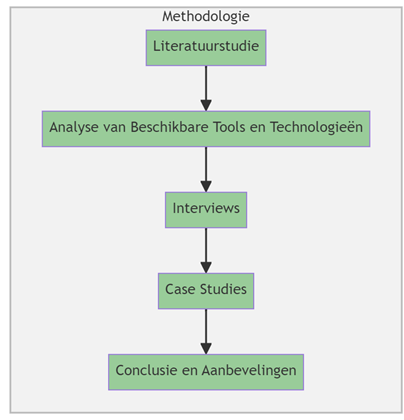
\includegraphics[width=\textwidth]{graphics/methodologie.png}
    \caption{...}
    \label{...}
\end{figure}


%---------- Verwachte resultaten ----------------------------------------------
\section{Verwachte Resultaten en Conclusie}%
\label{sec:verwachte-resultaten}

In de complexe wereld van ERP-downtime en patchmanagement in SAP ERP-systemen, spelen groot- en middelgrote bedrijven een cruciale rol in het handhaven van operationele efficiëntie te midden van technologische evoluties. De integratie van ERP-software is wijdverbreid en daarom ook vaak een doel van cyberaanvallen, hierdoor is er nood aan het tijdig patchen van beveiligingsrisico’s. 
Patchmanagementpraktijken variëren in organisatie tot organisatie, met enkele uitdagingen zoals trage updates en compatibiliteitsproblemen. Succes hangt af van factoren zoals proactieve benaderingen, geautomatiseerde tools en heldere communicatie.
Trends in SAP ERP wijzen op regelmatige updates en een verschuiving naar geautomatiseerde patchprocessen. Menselijke, technologische en organisatorische factoren blijken cruciaal in patchmanagement. Bewustwording, training, geavanceerde tools en samenwerking zijn sleutels tot succes. Aanbevelingen omvatten strategieën voor minimale impact op de continuïteit, effectieve communicatie en het verkennen van onbeantwoorde vragen in ERP-patching.
De voorgestelde bachelorproef onderscheidt zich door zijn holistische aanpak, die waardevolle inzichten en aanbevelingen belooft voor het optimaliseren van ERP-patchmanagement in groot- en middelgrote bedrijven.
